\chapter{Executing Supply Chain Scans with a Web Hook}\label{chap:build_env_affinity}


\section{Supply Chain Vulnerability Scans with \cxone}

Webhook integrations with \cxone are provided via the feedback applications.
Integration of \scaresolver for local execution is not currently available in
\cxone.


\section{Supply Chain Vulnerability Scans with CxFlow++}

\cxflow is a scan orchestration tool that is used for orchestrating scans for \cxsast and \cxsca.  One
of the typical methods of invoking scans is to received SCM webhook payloads to indicate when
a push or pull-request event occurs on a source code repository.  The required scan types are orchestrated,
and the results are posted to a pull request comment or issues tracker tickets are opened.

\cxflowplusplus is a re-packaged container image of \cxflow.  The configuration of \cxflow
does not change, but \cxflowplusplus adds some additional capabilities:

\begin{itemize}
    \item Advanced configuration options allow for pre-execution download of \cxflow configuration
    artifacts.
    \item Supply chain vulnerability scans via \scaresolver can be performed using
    \hyperref[sec:extending_environment]{build environment extension} container images with 
    affinity to the code targeted for the scan.
\end{itemize}

Figure \ref{fig:dispatcher_workflow} depicts the workflow of the dispatcher as it resolves
the \scaresolver execution environment that has affinity to a project with scans
orchestrated by \cxflowplusplus.  The scans are initiated by a web hook payload sent to the
\cxflowplusplus endpoint.  \cxsast scans are orchestrated in parallel with \cxsca scans by
\cxflowplusplus with the additional logic in the dispatcher.

Projects can be tagged to allow dispatcher to locate the correctly configured \scaresolver
container, as is demonstrated with Applications A and B in Figure \ref{fig:dispatcher_workflow}.
Application C and D may not be tagged for affinity with a specific container, so the
\scaresolver scan would be executed in a container configured with the \texttt{Default} tag.

\begin{figure}[h]
    \caption{\cxflowplusplus Dispatcher Workflow}
    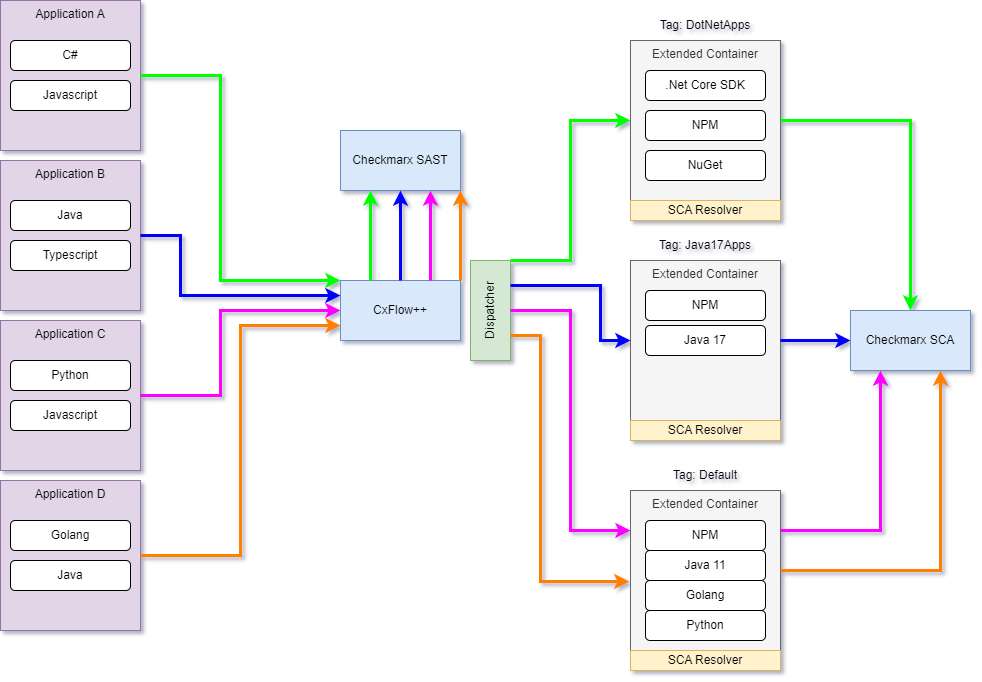
\includegraphics[width=\textwidth]{graphics/dispatcher_workflow.png}
    \label{fig:dispatcher_workflow}
\end{figure}


Some operational aspects of \cxflow may change when using \cxflowplusplus.  The \cxflowplusplus 
build environment affinity feature
\footnote{If there is no need to use this features of the dispatcher, \cxflowplusplus may not offer any advantages over \cxflow.} 
utilizes
\href{https://www.docker.com/blog/docker-can-now-run-within-docker/}{docker-in-docker (DIND)}; this may
change the compatibility of the runtime environment for an existing \cxflow deployment.

\subsection{\cxflowplusplus Runtime Environment}

The minimum recommended environment for \cxflowplusplus is:

\begin{itemize}
    \item 4 Cores
    \item 32 GB RAM
    \item 150GB of disk space
    \item Linux OS with kernel >= 5.12 if using \sysbox
\end{itemize}

\cxflowplusplus will be loading and executing container images as part of supply chain vulnerability scan
orchestration.  This can be potentially CPU and memory intensive.  Vertical or horizontal scaling
of \cxflowplusplus may be required to be able to orchestrate the volume of scans requested.

\noindent\\The execution of \cxflowplusplus must have some additional parameters provided to the
\texttt{docker} command to be able to create and execute docker containers inside the \cxflowplusplus
container.  If these additional parameters are not provided, \cxflowplusplus will emit errors when
attempting to execute docker containers inside the running container.

\subsubsection{DIND - Privileged Execution}

One method of enabling docker-in-docker is to execute containers in privileged mode.
Running \cxflowplusplus in privileged mode can be done like so:

\noindent\\\texttt{docker run -privileged -d ----restart unless-stopped \cxflowplusplustag}

\noindent\\\textbf{WARNING}
\noindent\\It is generally considered a bad security practice to run a docker container in privileged mode.
Given that some open source packages can execute malware payloads during dependency resolution, it is not
advised to run in privileged mode for production purposes.

\subsubsection{DIND - \sysbox Runtime}

An alternative to executing docker in privileged mode is to use \sysbox as a runtime.  \sysbox runs on Linux
and has a requirement of a kernel version >= 5.12.  Appendix \ref{chap:sysbox_install} has
a procedure that can be used to install \sysbox manually on a Linux OS.

\noindent\\\texttt{docker run ----runtime=sysbox-runc -d ----restart unless-stopped \cxflowplusplustag}

\subsection{Logging}

\cxflow logs to the console to maintain running compatibility with the official \cxflow image.  
Any supply chain vulnerability scan environment affinity operations are logged in files found
on the container in the directory \texttt{/var/log/dispatcher}.  To maintain the logs across
restarts of the container, it is recommended to map a local volume to \texttt{/var/log/dispatcher}.
The use of logging files for the dispatcher is to avoid the console logs from being corrupted
by spontaneous log emissions from the dispatcher.


\subsection{\cxflow Image Compatibility}

All the existing Spring Boot facilities for configuring \cxflow via environment variables work 
with the \cxflowplusplus image.  Using the \cxflowplusplus image in place of the official
\cxflow image is compatible as long as there is no need to execute \scaresolver.

If using \scaresolver, more configuration needed to provide a method of container image selection
for use in supply chain vulnerability scans.  The container will actively prevent
configuration of the \cxflow \texttt{SCA\_PATH\_TO\_SCA\_RESOLVER} option.  

The \cxflowplusplus image does not contain the \scaresolver runtime that would normally be found
in the official \cxflow image.  The \cxflowplusplus image replaces \scaresolver with
a mediation script known as \textit{the dispatcher} that invokes \scaresolver in an appropriate
container image.

The \cxflowplusplus image supports environment variables that change how it operates when 
preparing to start the \cxflow services.  Appendix \ref{chap:image_opts} has a complete list
of \cxflowplusplus additional options.


\subsection{\cxflow++ Dispatcher Configuration}




% The exact description of the Dispatcher is TBD.  The basic idea is to execute SCAResolver in a mostly sandboxed execution environment.  The execution environment
% could be a customized build environment.

% The execution environment can be defined as:

% * default - The default image, runtime parameters, environment variables, and SCAResolver parameters used if no runtime environment can be determined
% * tag - The image, runtime parameters, environment variables, and SCAResolver parameters used if a project has a matching tag

% Project tags are obtained from a config-as-code file in the root of the repository (not the CxFlow config-as-code file).  Future enhancements may allow this to be resolved from
% project tags found via the SCA API.






% ## Dispatcher Configuration

% Configuration can be represented by both YAML and Environment variables.  The first YAML file found in `$(pwd)/yaml` when the Dispatcher starts is used
% as the configuration file.  The configuration is evaluated in the following order of precedence:

% 1. Environment variables
% 2. YAML configuration

% An example of the complete YAML configuration can be observed below:

% ```yaml

% docker:
%     login:
%         registry-1.docker.io:
%             username: XXXXXXXXX
%             password: XXXXXXXXX
%         ...
%         ghcr.io:
%             username: XXXXXXXXX
%             password: XXXXXXXXX

% resolver:
%     defaults:
%         containerttl: 15m
%         exectimeout: 10m
%         defaulttag: default

%     images:
%         default:
%             container: test:gradle
%             containerttl: 5m
%             exectimeout: 10m
%             execenv:
%                 FOO: BAZ
%             execparams:
%                 - --log-level=Verbose
%         node: 
%             container: test:node-linux
%             execenv:
%                 FOO: BAR
%             envpropagate:
%                 - MY_ENVIRONMENT_VARIABLE1
%                 - MY_ENVIRONMENT_VARIABLE2

% ```


% ### Section: `docker`

% This section is optional.  It is intended to provide defaults for Docker invocations.

% #### `docker.login`

% This section is a list of container repositories where a `docker login` command will be executed on CxFlow startup.  If the images tags
% configured in the `resolver` section are not stored in the default Docker public repository, configure the repositories here.

% Multiple image repositores can be defined using multiple entries under `docker.login`.


% ```yaml

% docker:
%     login:
%         registry-1.docker.io:
%             username: XXXXXXXXX
%             password: XXXXXXXXX
%         ghcr.io:
%             username: XXXXXXXXX
%             password: XXXXXXXXX
%         my-host.com:
%             username: XXXXXXXXX
%             password: XXXXXXXXX
% ```

% Dashes in hostnames can be represented in environment variable names with a double underscore.  Underscores are not valid in DNS hostnames and are therefore not supported.

% The above example of the `docker.login` YAML has the equivalent environment variables:

% ```
% DOCKER_LOGIN_HUB_DOCKER_IO_USERNAME=XXXX
% DOCKER_LOGIN_HUB_DOCKER_IO_PASSWORD=XXXX
% DOCKER_LOGIN_MY__HOST_COM_USERNAME=XXXX
% DOCKER_LOGIN_MY__HOST_COM_PASSWORD=XXXX
% ```


% ### Section: `resolver`

% This section is used to define parameters for SCAResolver invocation.

% #### `resolver.twostage`

% This is optional, defaults to `true`.

% If `true`, an `online` SCAResolver scan will be split into two stages:

% * The first stage is an `offline` scan.  When invoking the offline scan, credentials for the SCA server are stripped from the command.  This executes the dependency
% resolution without leaving credentials exposed to any scripts that execute as part of the dependency resolution.
% * The second stage is an `upload` where the dependency resolution results are uploaded to the SCA server.

% If set to `false`, an `online` scan will be invoked in a single step.


% #### `resolver.defaults`

% This section is optional; it allows for overriding the hard-coded default values if desired.

% The timespan values here can be represented by simple value strings with numeric indicators indicating time units such as `h` for hours, `m` for 
% minutes, and `s` for seconds.  Example:

% `2h15m30s` means 2 hours, 15 minutes, and 30 seconds

% `15m` means 0 hours, 15 minutes, and 0 seconds

% An example of the `resolver.defaults` section can be observed below:

% ```yaml

% resolver:
%     defaults:
%         containerttl: 15m
%         exectimeout: 10m
%         defaulttag: default
%         delete: False

% ```

% `resolver.defaults.containerttl` - If not provided, this defaults to 1 hour.  This is the length of time a container image will be used after the
% initial `docker pull` command is executed to download the image.  This allows updated images to be retrieved without the need to stop CxFlow.

% `resolver.defaults.exectimeout` - If not provided, this defaults to 30 minutes.  This is the amount of time CxFlow will allow the SCAResolver
% image to execute before killing it and assuming failure.

% `resolver.defaults.defaulttag` - If not provided, this defaults to the value of `default`.  This is the tag of the image configured in
% `resolver.images` used if an unknown tag is requested.

% `resolver.defaults.delete` - If not provided, this defaults to the value of `True`.  Setting this to `False` will prevent the container image created
% for the scan from being deleted.

% The above example of the `resolver.defaults` YAML has the equivalent environment variables:

% ```
% RESOLVER_DEFAULTS_CONTAINTERTTL=15m
% RESOLVER_DEFAULTS_EXECTIMEOUT=10m
% RESOLVER_DEFAULTS_DEFAULTTAG=default
% RESOLVER_DEFAULTS_DELETE=False
% ```

% #### `resolver.images`

% This section is where the image parameters are set for a container matching a tag that indicates which container image to
% use when invoking SCAResolver.

% Each dictionary of key/value pairs configured under the `resolver.images` uses the key value as the image tag.  An example of a configuraton
% for images tagged `default` and `node`.  The containers defined would be instances of [the SCAResolver sandbox](../sandbox) image derived
% from an appropriate build environment base image.

% In each of the sections, the `containerttl` and `exectimeout` values are optional.  If not provided, the corresponding values from the 
% `resolver.defaults` section will be used.


% ```yaml

% resolver:
%     images:
%         default:
%             container: test:gradle
%             containerttl: 5m
%             exectimeout: 10m
%             execenv:
%                 FOO: BAZ
%             execparams:
%                 - --log-level=Verbose
%         node: 
%             container: test:node-linux
%             execenv:
%                 FOO: BAR
%             envpropagate:
%                 - MY_ENVIRONMENT_VARIABLE1
%                 - MY_ENVIRONMENT_VARIABLE2

% ```


% `resolver.images.<tag>.container` - Required.  The container image tag name associated with the configuration tag that will be resolved as
% part of the CxFlow scan execution.  

% `resolver.images.<tag>.containerttl` - Optional.  Uses the corresponding value from `resolver.defaults` if not provided.

% `resolver.images.<tag>.exectimeout` - Optional.  Uses the corresponding value from `resolver.defaults` if not provided.

% `resolver.images.<tag>.execenv` - Optional.  A dictionary of key/value pairs that are emitted in the environment when the container image is executed.  Entries
% with key values that match keys defined in `resolver.images.<tag>.envpropagate` will have the value overwritten by the value found in the propagated environment
% value.

% `resolver.images.<tag>.execparams` - Optional.  An array of values passed to SCAResolver at the end of all other parameters needed to control the
% execution of SCAResolver.  The values here are mainly intended to pass configuration values to dependency resolution tools invoked by SCAResolver.  Passing other values
% to SCAResolver may cause operational conflicts.

% `resolver.images.<tag>.envpropagate` - Optional.  An array of names of environment variables in the CxFlow environment that will be propagated as-is to the 
% executing image environment.

% `resolver.images.<tag>.dockerparams` - Optional. An a key/value dictionary that follows the `**kwargs` key/value pairs supported in the [Docker Python API](https://docker-py.readthedocs.io/en/stable/containers.html#docker.models.containers.ContainerCollection.run) `run` method.


% The above example of the `resolver.images` YAML has the equivalent environment variables:

% ```
% RESOLVER_IMAGES_DEFAULT_CONTAINER=test:gradle
% RESOLVER_IMAGES_DEFAULT_CONTAINERTTL=5m
% RESOLVER_IMAGES_DEFAULT_EXECTIMEOUT=10m
% RESOLVER_IMAGES_DEFAULT_EXECENV_FOO=BAZ
% RESOLVER_IMAGES_DEFAULT_EXECPARAMS_1=--log-level=Verbose
% RESOLVER_IMAGES_NODE_CONTAINER=test:node-linux
% RESOLVER_IMAGES_NODE_EXECENV_FOO=BAR
% RESOLVER_IMAGES_NODE_ENVPROPAGATE_1=MY_ENVIRONMENT_VARIABLE1
% RESOLVER_IMAGES_NODE_ENVPROPAGATE_2=MY_ENVIRONMENT_VARIABLE2
% ```

% ## Resolving the Tag for an SCA Scan

% When an SCA scan is invoked, the `default` image tag is used unless a config-as-code file is provided that explicitly
% defines the image tag to use when executing SCAResolver.

% The config-as-code file named `.cxsca` should be placed in the root of the repository.  The contents should be:

% ```json
% {
%     "version" : "1",
%     "tag" : "<image tag>"
% }
% ```
